\documentclass[14pt]{article}
%General Packages
\usepackage{multicol, enumerate, enumitem, hyperref, color, soul, setspace, parskip, fancyhdr}

%Math Packages
\usepackage{amssymb, amsthm, amsmath, bbm, latexsym, units, mathtools}

%All math in Display Style
\everymath{\displaystyle}

% Packages with additional options
%\usepackage[T1]{fontenc}
\usepackage[headsep=0.5cm,headheight=0cm, left=1 in,right= 1 in,top= 1 in,bottom= 1 in]{geometry}
\usepackage[usenames,dvipsnames]{xcolor}

% SageTeX
\usepackage{sagetex}

% Package to use the command below to create lines between items
\usepackage{dashrule}
\newcommand{\litem}[1]{\item#1\hspace*{-1cm}\rule{\textwidth}{0.4pt}}

\pagestyle{fancy}
\lhead{Module\,7\,-\,Rational\,Functions}
\chead{}
\rhead{Progress Exam 3}
\lfoot{Summer\,C\,2020}
\cfoot{}
\rfoot{Version B}

\begin{document}
\pagestyle{fancy}

\begin{sagesilent}
load("../Code/generalPurposeMethods.sage")
load("../Code/keyGeneration.sage")
keyFileName = "Module7"
version = "B"
\end{sagesilent}

\begin{enumerate}
\setcounter{enumi}{30}


\begin{sagesilent}
moduleNumber=7
problemNumber=31
load("../Code/rational/solveRationalLinear.sage")
\end{sagesilent}

\litem{ \sage{displayStem}

	\[ \sage{leftSide} = \frac{\sage{factorNumerator3}}{\sage{factorDenominator3}}  \]

	\begin{enumerate}[label=\Alph*.]
    \item \( \sage{choices[0]} \)
    \item \( \sage{choices[1]} \)
    \item \( \sage{choices[2]} \)
    \item \( \sage{choices[3]} \)
    \item \( \sage{choices[4]} \)
	\end{enumerate}
}

\begin{sagesilent}
moduleNumber=7
problemNumber=32
load("../Code/rational/domainRational.sage")
\end{sagesilent}

\litem{ \sage{displayStem}

\[ \sage{displayProblem} \]

	\begin{enumerate}[label=\Alph*.]
		\item \( \sage{choices[0]} \)
		\item \( \sage{choices[1]} \)
		\item \( \sage{choices[2]} \)
		\item \( \sage{choices[3]} \)
		\item \( \sage{choices[4]} \)
	\end{enumerate}
}

\begin{sagesilent}
moduleNumber=7
problemNumber=33
load("../Code/rational/rationalEquationToGraph.sage")
\end{sagesilent}

\litem{ \sage{displayStem}
\[ \sage{displayProblem} \]

	\begin{enumerate}[label=\Alph*.]
\begin{multicols}{2}
		\item \begin{center}
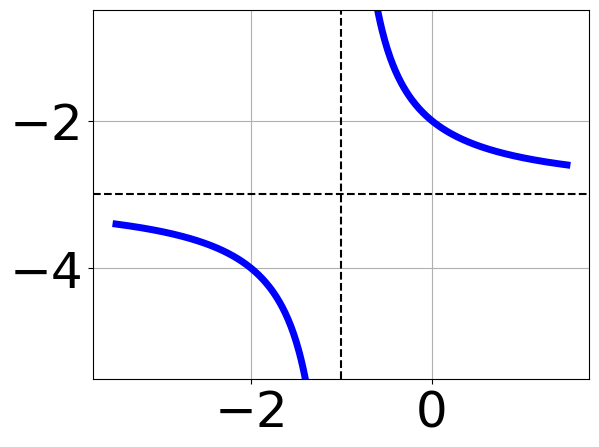
\includegraphics[width=.3\textwidth]{../Figures/rationalEquationToGraphBA.png}
\end{center}
		\item \begin{center}
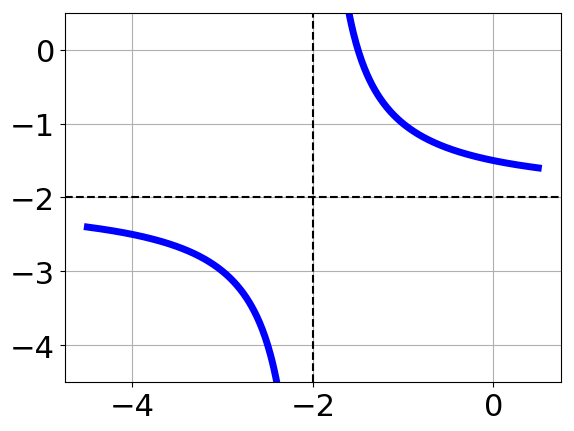
\includegraphics[width=.3\textwidth]{../Figures/rationalEquationToGraphBB.png}
\end{center}
\columnbreak
		\item \begin{center}
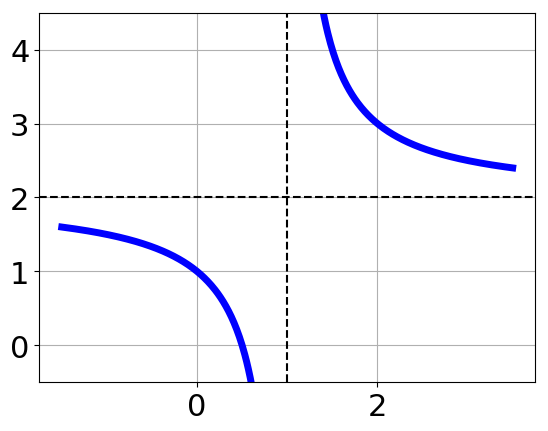
\includegraphics[width=.3\textwidth]{../Figures/rationalEquationToGraphBC.png}
\end{center}
		\item \begin{center}
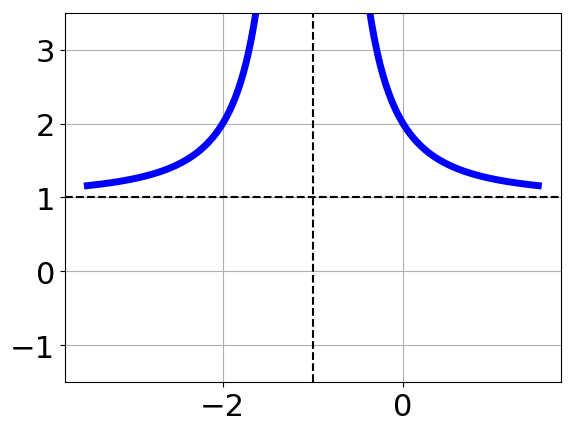
\includegraphics[width=.3\textwidth]{../Figures/rationalEquationToGraphBD.png}
\end{center}
\item \text{None of the above.}
\end{multicols}
	\end{enumerate}
}

\begin{sagesilent}
moduleNumber=7
problemNumber=34
load("../Code/rational/solveRationalQuadratic.sage")
\end{sagesilent}

\litem{ \sage{displayStem}

	\[ \sage{displayProblem} \]

	\begin{enumerate}[label=\Alph*.]
    \item \( \sage{choices[0]} \)
    \item \( \sage{choices[1]} \)
    \item \( \sage{choices[2]} \)
    \item \( \sage{choices[3]} \)
    \item \( \sage{choices[4]} \)
	\end{enumerate}
}

\begin{sagesilent}
moduleNumber=7
problemNumber=35
load("../Code/rational/rationalGraphToEquation.sage")
\end{sagesilent}

\litem{ \sage{displayStem}

\begin{multicols}{2}
\begin{center}
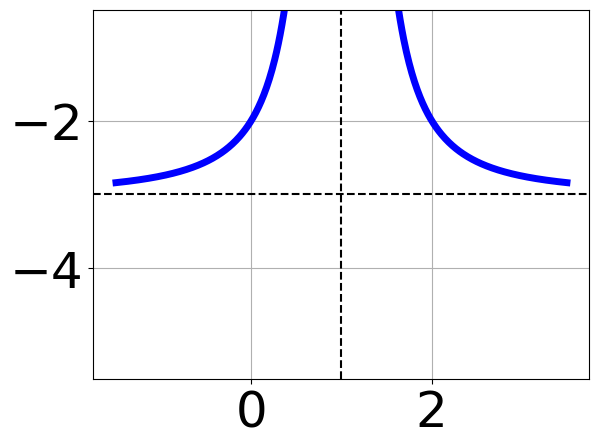
\includegraphics[width=.3\textwidth]{../Figures/rationalGraphToEquationB.png}
\end{center}

\columnbreak

	\begin{enumerate}[label=\Alph*.]
		\item \( \sage{choices[0]} \)
		\item \( \sage{choices[1]} \)
		\item \( \sage{choices[2]} \)
		\item \( \sage{choices[3]} \)
    \item None of the above
	\end{enumerate}
\end{multicols}
}

\end{enumerate}

\end{document}

